\chapter{Moyens d'identification}
Dans ce chapitre, nous allons nous intéresser aux techniques qui permettent de tracer les utilisateurs. Plus précisément, nous allons voir comment ces techniques utilisent ou détournent les mécanismes assurant le fonctionnement du Web.

\section{Imperfections du principe de même origine}
\label{imperfections_sop}
L'échec de la bonne adaptation de ce principe est une source importante de fuites de données et d'attaques. Les violations du principe de même origine peuvent être dues à un filtrage de script insuffisant du côté des applications Web du serveur ou à des défauts dans les mécanismes d'isolation des domaines au sein du navigateur \cite{Chen:2007:ABD:1315245.1315248}.

Les défauts de filtrage des scripts au niveau des serveurs sont communément appelés failles XSS (\textit{cross-site scripting}). En exploitant ces failles, des scripts malveillants peuvent passer à travers le filtrage et être exécutés dans le même contexte de sécurité que les applications Web authentiques.

Au niveau des navigateurs Web, les violations du principe de même origine sont dues à une mauvaise isolation des contenus des différents domaines. Certains domaines peuvent alors accéder aux informations appartenant à d'autres domaines alors qu'ils ne devraient pas y avoir accès.
\newline

Lorsqu'un attaquant désire compromettre une application, il est parfois plus facile d'attaquer les utilisateurs à travers leur navigateur Web que le serveur lui-même \cite{sullivan2011web}. Les navigateurs sont défendus par le principe de même origine mais la présence de failles dans le site Web ou dans le serveur peuvent permettre à l'attaquant de passer outre ce principe. La principale vulnérabilité des sites sont les attaques XSS. Celles-ci consistent en une vulnérabilité qui permet à un attaquant de placer son code au sein des pages d'une application Web vulnérable. Lorsqu'un visiteur se rend sur l'une de ces pages, le code de l'attaquant est chargé avec les autres éléments de la page. Ce script malicieux peut alors en être en mesure de lire le cookie de l'utilisateur ou récupérer des valeurs affichées uniquement à l'utilisateur en utilisant du JavaScript. Ensuite, une requête HTTP contenant les données volées serait utilisée afin de les envoyer au serveur de l'attaquant. Celui-ci sera ensuite capable de se faire passer pour l'utilisateur légitime sur le site ou d'utiliser les informations reçues à mauvais escient (il pourrait par exemple s'agir de données bancaires), voir \autoref{exemple_XSS}.
\newline

\begin{figure}[h]
	\centering
	\begin{lstlisting}
<script>
  // Vol du numero de client
  var numeroDuClient = document.getElementById('numClient').innerHTML;
  // Vol du cookie
  var cookieDuClient = document.cookie;
  // Requete contenant les informations volees :
  var requete = 'http://serveur-du-voleur.be/vol?client=' + numeroDuClient + '&cookie=' + cookieDuClient;
  // Envoi de la requete avec une image
  document.write("<img src='" + requete + "'/>");
</script>
	\end{lstlisting}
	\caption{\label{exemple_XSS}Un exemple d'attaque XSS pour voler des informations.}.
\end{figure}
Quand le client va se rendre sur la page, son navigateur va automatiquement faire une requête vers le serveur du voleur. Son navigateur l'avertira seulement que l'image n'a pas été trouvée mais les informations auront été néanmoins transmises au voleur. Cette attaque nécessite un minimum de préparation car le voleur doit savoir quel est le nom ou l'ID de l'élément HTML qui affiche le numéro de client (dans l'exemple, "numClient").
Ceci est un premier exemple de violation du principe de même origine réalisé avec l'aide d'une faille XSS.
\newline

Il existe plusieurs moyens de contourner le principe de même origine. Le but de ce chapitre n'étant pas d'en faire une liste exhaustive, seuls quelques moyens seront expliqués.
Il faut également préciser que même si le principe était correctement implémenté au sein d'un navigateur, il n'empêcherait pas les violations de vie privée face à des sites coopérants. Ceci s'explique par le fait qu'il existe une multitude de techniques simples allant des redirections jusqu'aux liens inter-sites pouvant être utilisées dans le but de transmettre des données entre des sites. Avec de tels échanges, les sites coopérants sont dans la capacité de constituer un profil inter-domaine des activités de leurs visiteurs.
%\newline

%La possibilité de violer le principe de même origine est la source de nombreuses méthodes qui permettent de tracer les utilisateurs. En effet, elle permet à un site A de créer et récupérer un cookie sur l'ordinateur de l'utilisateur s'il visite un autre site B qui inclut du contenu du site A (\autoref{cookies}). Cela autorise également des sites à accéder à des éléments d'un autre site enregistrés en cache (\autoref{cache}).

%L'absence d'implémentation du principe de même origine dans l'historique de l'utilisateur permet de déterminer si le navigateur a été utilisé pour visiter un site en regardant la couleur des liens hypertextes pointant vers ce site. Dans ce cas, l'utilisation de cookies n'est même plus nécessaire.
%\newline

%Le traçage des utilisateurs peut être classé en plusieurs catégories \cite{Jackson:2006:PBS:1135777.1135884} :
%\begin{itemize}
%  \item tracking sur une seule session : inévitable vu comment le Web fonctionne
%  \item tracking sur de multiples sessions : permet à un site d'identifier un visiteur s'il revient plus tard sur le site
%  \item tracking coopératif : permet à des sites coopérants de créer un historique des visites d'un utilisateur sur tous les sites de la coopération
%  \item tracking semi-coopératif sur un seul site : permet à un site de déterminer des informations sur les activités d'un visiteur sur un autre site en y plaçant du contenu (par exemple, en plaçant une image sur un forum)
%  \item tracking semi-coopératif sur de multiples sites : identique au tracking semi-coopératif sur un seul site à l'exception qu'il peut y avoir plusieurs sites ciblés
%  \item tracking non coopératif : permet à un site de déterminer des informations sur les activités d'un visiteur sur un autre site sans participation du site ciblé
%  \newline
%\end{itemize}
%
%Certains types de tracking peuvent être évités en améliorant le principe de même origine mais il est malheureusement difficile de contrer les types de tracking dits coopératifs.

%%%%%%%%%%%%%%%%%%%%%%%%%%%%%%
\section{Cookies}
\label{cookies}
En général, on utilise deux types de classification pour les cookies \cite{Yue:2007:ACU:1251984.1253093}.

Le premier se base sur l'origine et la destination : les cookies sont classifiés en tant que cookies "first-party" ou "third-party". Les cookies "first-party" sont issus du domaine que l'utilisateur est en train de visiter, on les appelle cookies d'origine ou cookies de domaine. Les cookies "third-party" sont créés par un site autre que celui qui est visité par l'utilisateur, on les appelle cookies tiers.\\
Les cookies tiers sont placés suite à des réponses HTTP venant de sites tiers. Un site \textit{alpha.com} ne peut pas créer de cookie au nom du site \textit{beta.com} (voir RFC 6265 \cite{IETF_RFC6265}, section 4.1.2.3), cela provoquerait des problèmes de sécurité évidents. Pour les mêmes raisons, les cookies ayant un suffixe public \footnote{Un suffixe public est un domaine qui est contrôlé par un registre public comme "com", "co.uk" ou "pvt.k12.wy.us" \cite{IETF_RFC6265}. Une liste est maintenue par le projet Mozilla : \url{http://publicsuffix.org/}.} dans l'attribut \textit{Domain} sont rejetés.

La seconde méthode de classification se base sur la durée de vie du cookie : les cookies sont alors classifiés en cookies de session ou cookies persistants. Les cookies de session sont stockés dans la mémoire vive de l'ordinateur et supprimés à la fermeture du navigateur. A l'opposé, les cookies persistants sont stockés sur le disque dur de l'ordinateur et supprimés soit lors de leur expiration, soit manuellement par l'utilisateur.
\newline

Les cookies tiers, qu'ils soient de session ou persistants, n'apportent quasiment aucun bénéfice à l'utilisateur. Ils sont d'ailleurs reconnus comme une menace pour la vie privée et les navigateurs proposent généralement une option pour les désactiver.

Les cookies d'origine de type session ne posent généralement pas vraiment de problèmes relatifs à la vie privée étant donné leur faible durée de vie. En théorie, ceci est valable car l'utilisateur ferme les fenêtres de son navigateur régulièrement. Par contre, un utilisateur qui laisse constamment l'onglet d'un site ouvert pourrait se faire tracer par le site en question.

A l'opposé, les cookies d'origine persistants peuvent poser des problèmes divers. En effet, les cookies persistants sont une arme à double tranchant : ils peuvent jouer un rôle utile en permettant la personnalisation et l'authentification sur les sites mais ils peuvent également jouer un rôle plus dangereux qui amène des risques au niveau de la vie privée et de la sécurité. Ces risques reposent sur deux aspects : le premier, et celui qui nous intéresse principalement ici, est que les cookies persistants permettent de tracer l'activité de l'utilisateur dans le temps. En effet, pour chaque page visitée, le client envoie une requête au serveur, celui-ci est donc capable de suivre l'utilisateur lors de la visite du site. Le deuxième risque est que les cookies persistants peuvent être volés ou manipulés par des attaques de deux types : les attaques XSS (elles exploitent les vulnérabilités des applications Web, voir la \autoref{exemple_XSS} de la \autoref{imperfections_sop}) et les attaques qui exploitent les vulnérabilités des navigateurs Web (via notamment le contournement du principe de même origine).
\newline

Une étude menée sur plus de 5000 sites à propos de l'utilisation des cookies \cite{Yue:2007:ACU:1251984.1253093} a montré que les cookies d'origine persistants sont largement utilisés et que plus de 60\% sont réglés pour expirer plus d'un an après leur création.
\newline

Désactiver tous les cookies tiers et garder les cookies d'origine de type session est supporté par la majorité des navigateurs actuels. Le problème se situe au niveau des cookies d'origine persistants car on ne sait pas comment les gérer et déterminer s'ils sont utiles ou néfastes pour l'utilisateur.

%- parler des cookies de cache dans la section cookies ou dans la section cache ?

%%%%%%%%%%%%%%%%%%%%%%%%%%%%%%
\section{Cache}
\label{cache}
Le cache du navigateur permet d'enregistrer localement une copie des fichiers afin de ne pas devoir les recharger lors d'une visite ultérieure. Ce mécanisme est très utile car il permet d'économiser de la bande passante et du temps. Cependant, il donne la possibilité à des sites web de déterminer si leurs visiteurs ont visité un autre site auparavant.

\subsection{Tracking par mesure du temps}
Une méthode d'exploitation du cache à des fins de surveillance est détaillé par Felten et Schneider \cite{Felten:2000:TAW:352600.352606}.
Le principe est assez simple : il exploite le fait qu'un fichier présent en cache sera chargé beaucoup plus rapidement qu'un fichier qui ne l'est pas. Donc en mesurant le temps d'accès au fichier, il est possible de déterminer si une personne a déjà visité le site web (ou plus précisément, la page) qui utilise ce fichier. En effet, rien n'empêche un site web de charger un fichier hébergé par un autre site.
\newline

Imaginons que l'administrateur d'un site \emph{(alpha.com)} veuille savoir si ses visiteurs se sont également rendus sur un autre site \emph{(beta.com)}. La première chose qu'il doit faire est de se rendre sur le site qu'il veut cibler et choisir un fichier statique pouvant être mis en cache et qui est chargé par tout visiteur (un logo par exemple). Ensuite, le but est de mesurer le temps d'accès du fichier cible.

Le plus fiable et facile est d'utiliser un applet Java ou un JavaScript qui va mesurer le temps de chargement du fichier à partir de son URL. Même si l'utilisateur a désactivé l'exécution de Java et de JavaScript, il est possible d'obtenir une mesure suffisamment précise en chargeant les fichiers suivants dans l'ordre :

\begin{enumerate}
  \item un fichier du site \emph{alpha.com}
  \item le fichier cible du site \emph{beta.com}
  \item un autre fichier du site \emph{alpha.com}
\end{enumerate}

En soustrayant les moments auxquels le serveur reçoit les requêtes des fichiers 1 et 3, l'administrateur du site \emph{alpha.com} est en mesure d'avoir une approximation du temps qu'il a fallu pour charger le fichier 2 (celui de \emph{beta.com}).

Il faut néanmoins respecter certains critères pour que cela fonctionne : forcer le chargement des fichiers de manière séquentielle et de manière invisible en n'altérant pas l'apparence de la page afin que le client ne remarque rien.
\newline

Il est possible d'améliorer la probabilité de distinguer correctement les succès des défauts de cache en effectuant différentes mesures, ce qui permet alors de raffiner les seuils de discrimination : refaire plusieurs fois la mesure d'un même fichier (à partir de la seconde tentative, le fichier sera présent dans le cache) pour les succès de cache et utiliser l'URL de fichiers n'existant pas pour les défauts de cache.

Afin d'améliorer la précision, il est également intéressant de combiner les résultats de plusieurs fichiers mesurés individuellement.
\newline

D'une manière semblable, ce type d'attaque peut également être réalisé sur le cache du DNS. Felten et Schneider ont vérifié la précision des tests avec l'aide de 3 serveurs distincts situés à des distances différentes.

Plus le serveur est situé à une grande distance, plus la requête DNS prend de temps. Les tests ont montré que la précision des résultats pouvait être inférieure car la pénalité suite à des défauts de cache était très petite. Il n'était donc pas possible de discriminer les échecs des succès de cache. Cependant, sur Internet, la pénalité en cas de défaut est suffisamment grande pour assurer une bonne distinction. Dans ce cas-là, les tests montrent une très bonne précision.
\newline

% Attache de cookies de cache

Cette attaque peut être menée dans différentes situations :
\begin{itemize}
  \item Un site web qui veut en savoir davantage sur ses visiteurs.
  \item Une régie publicitaire pourrait inclure le code de mesure dans les bannières qu'elle distribue afin de faire des statistiques sur les sites web consultés par les visiteurs.\\Il est même possible de distribuer un code différent pour les catégoriser.\\Bien entendu, cette attaque résulte d'une collaboration entre le site et la régie publicitaire.
  \item L'attaquant pourrait créer un site web de telle façon à ce qu'il apparaisse en tête des moteurs de recherche dans le but de faire des statistiques sur les personnes intéressées par un sujet particulier. Il faut noter que cette situation reste théorique et a peu de chances de fonctionner.
  \item L'attaquant pourrait envoyer un mail contenant le code HTML à sa victime.\\En le faisant ressembler à du spam, la victime ne remarquerait rien d'anormal et la mesure serait effectuée.
\end{itemize}

% Timing Attacks on Web Privacy (section 1) : raisons de s'inquiéter
% Timing Attacks on Web Privacy (section 7) : contre-mesures actuelles sont inefficaces
% Timing Attacks on Web Privacy (section 8) : solution possible

\subsection{Stockage local HTML5}
\label{cache_html5}
Une nouveauté d'HTML5 est la possibilité de stocker localement des données pour un usage hors-ligne \cite{West:2012:APS:2038772.2038791}.
Le stockage local pourrait servir de "super-cookie" car il permet de stocker jusqu'à 5MB de données. De plus, ces données sont dites persistantes car elles doivent être supprimées par l'utilisateur ou le site Web.
\newline

Dans une expérience portant à l'origine sur le traçage via les cookies Flash \cite{flash_cookies_privacy_2} (voir \autoref{flash}), les chercheurs ont ajouté cette nouvelle dimension apportée par l'HTML5.
L'expérience réalisée une première fois en 2009 portait sur les cookies Flash et les cookies HTTP. Une expérience similaire a été réalisée à nouveau en 2011 en apportant également des informations relatives au stockage permis par l'HTML5.
\newline

Les analyses ont été réalisées sur le TOP 100 donné par Quantcast \footnote{Quantcast est une entreprise spécialisée dans la mesure d'audience et la publicité.} en juillet 2011.
Il en ressort que 17 sites sur les 100 ont utilisé le stockage local HTML5 pour un total de 60 paires clé-valeur. Les chercheurs ont trouvé des correspondances entre le stockage local HTML5 et les cookies HTTP dans différents cas (\textit{twitter.com}, \textit{tmz.com}, \textit{squidoo.com}, \textit{nytimes.com}, \textit{hulu.com}, \textit{foxnews.com} et \textit{cnn.com}). Dans la plupart de ces cas, la valeur commune aux deux éléments était issue d'un service tiers (comme \textit{meebo.com}, \textit{kissanalytics.com} et \textit{polldaddy.com}).

\subsection{ETags}
\label{cache_etags}
Le champ d'entête \textit{ETag} est défini dans la RFC 2616 \cite{IETF_RFC2616}. Il permet de déterminer si l'élément présent en cache dans le navigateur correspond à celui présent sur le serveur. Il est choisi arbitrairement par le serveur et est placé dans les réponses HTTP. Lorsqu'un client fait une requête vers un serveur et qu'il possède une copie du fichier en cache avec son \textit{ETag}, le serveur va comparer les deux \textit{ETags}. Cela permet d'économiser de la bande passante car le serveur n'envoie pas l'élément si les deux \textit{ETags} correspondent. Un exemple est disponible à la \autoref{etag} \footnote{Exemple tiré de \url{http://www.w3.org/2005/MWI/BPWG/techs/CachingWithETag.html}}.
\begin{figure}[h]
	\centering
	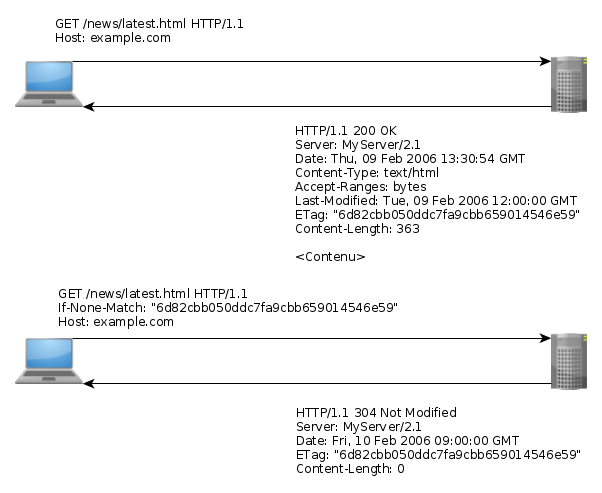
\includegraphics[scale=0.55]{figures/ETag.png}
	\caption{\label{etag}Un exemple de requêtes et réponses HTTP utilisant l'\textit{ETag}.}
\end{figure}
\newline

Dans l'expérience mentionnée dans la \autoref{cache_html5} et expliquée dans la \autoref{flash}, les chercheurs ont trouvé un cas de réapparition de cookie HTTP (un cookie HTTP a été supprimé par l'utilisateur puis un cookie identique a été recréé grâce au stockage local HTML5) sur \textit{hulu.com} à travers un service hébergé sur \textit{kissmetrics.com}. La technique a utilisé les ETags afin de sauvegarder les valeurs.
\newline

D'après les chercheurs, le tracking via l'entête ETag et le fait de pouvoir récréer des cookies à l'identique est particulièrement problématique car cette technique génère des valeurs de tracking uniques même si l'utilisateur bloque les cookies HTTP et Flash. En effet, afin d'empêcher ce traçage, l'utilisateur devrait vider son cache entre chaque site visité. De plus, en mode de navigation privée, l'utilisateur peut quand même être suivi durant une même session.

%%%%%%%%%%%%%%%%%%%%%%%%%%%%%%
\section{Pixels espions}
Les pixels espions sont des images de taille minime (généralement, de 1 pixel de haut sur 1 pixel de large) et sont destinés à effectuer une requête HTTP vers un serveur sans que le visiteur de la page ne s'en aperçoive. L'administrateur du site hébergeant ce pixel espion peut dès lors analyser les logs de son serveur Web afin d'obtenir des informations sur l'utilisateur. En plaçant un pixel espion spécifique sur chaque site, il est possible de distinguer sans problème les requêtes provenant des différents sites et ainsi déterminer quel site a été visité par chaque utilisateur.
En analysant la requête envoyée par le client, le serveur peut connaître plusieurs informations : la date et l'heure à laquelle le visiteur s'est rendu sur la page, son "User-Agent" (le navigateur utilisé, sa version, le système d'exploitation...), la langue, les cookies et toutes les informations disponibles par défaut dans une requête HTTP.\\
De plus, l'URI présente dans celle-ci peut contenir des informations additionnelles placées dans la requête de l'URI (après le point d'interrogation), voir la \autoref{exemple_XSS}.
\newline

Les pixels espions sont généralement utilisés pour tracker les visites. Par exemple, un site commercial pourrait placer un pixel de tracking sur sa page de confirmation d'achat. Cela enverrait alors une requête vers un serveur qui analyse les requêtes reçues et le parcours de l'acheteur pourrait être retracé avec l'information contenue dans le cookie. Par exemple, un cookie pourrait contenir le nom de la campagne de publicité qui a amené le visiteur sur le site. Les statistiques reçues permettraient alors au site de déterminer quelle campagne marketing a le mieux fonctionné.

%%%%%%%%%%%%%%%%%%%%%%%%%%%%%%
\section{JavaScript}
JavaScript permet d'exécuter des scripts du côté client. Il a entraîné le déploiement d'applications riches et accessibles simplement via un navigateur Web. Les possibilités sont multiples : il est ainsi facile de se divertir grâce à un jeu écrit en JavaScript mais il est également aisé d'en savoir plus sur l'utilisateur via le navigateur qui exécute le script. Ceci est possible grâce à l'accès dont dispose JavaScript sur l'ordinateur du client. En effet, différents attaques peuvent être perpétrées avec JavaScript afin d'identifier les utilisateurs \cite{Jang:2010:ESP:1866307.1866339}.
\newline

\begin{itemize}
	\item Le vol de cookies : le script inclus depuis un site tiers a accès à toutes les informations présentes sur la page. Lorsque celle-ci fait appel à un script, elle lui donne accès aux cookies, à la barre d'adresses et à l'ensemble des éléments disponibles sur la page. Le script a donc la capacité de lire le contenu des cookies associés au site et de l'envoyer à un site tiers (une régie publicitaire par exemple).
	\item Le détournement d'adresse : le script, ayant l'accès complet au contenu de la page, peut influencer les valeurs des URL. Le script peut également rediriger le navigateur vers un autre site et le rediriger ensuite vers le site d'origine sans que l'utilisateur ne s'en aperçoive (au chargement de la page par exemple).
	\item L'analyse de l'historique : l'attaque consiste à regarder comment les liens sont affichés par le navigateur. En effet, s'ils ont été visités, les liens s'affichent d'une autre couleur. Avec JavaScript, il suffit alors de créer un lien vers le site que l'on désire cibler dans une partie invisible de la page et utiliser l'interface DOM du navigateur pour regarder comment celui-ci affiche le lien. Cette attaque est possible car dans la plupart des navigateurs, l'accès à un historique de pages visitées, de fichiers cachés et de cache DNS est partagé entre les domaines. Cependant, ces éléments ne sont pas accessibles simplement : par exemple, il est nécessaire de placer un lien vers un site pour accéder à l'information concernant ce site et pouvoir déterminer s'il a été visité grâce à la couleur du lien affiché.
	\item Le traçage de comportement : il est possible de déterminer avec précision le comportement de l'utilisateur sur la page qu'il visite. L'élaboration d'une ligne du temps avec les interactions de l'utilisateur (clics, mouvements, défilements, parties de texte surlignées,...) est réalisable avec l'aide de gestionnaires d'événements. Cet ensemble d'interactions peut alors être envoyé à un site tiers afin de calculer des statistiques sur la navigation de l'utilisateur.
	\newline
\end{itemize}

Lorsque du code JavaScript est inclus dans une page, il n'est pas soumis au principe de même origine (\autoref{sop}). Ce script a donc accès à l'ensemble des éléments de la page et pourrait potentiellement récupérer des données, voir \autoref{inclusion_js}. \cite{sullivan2011web}.
\begin{figure}[h]
	\centering
	\begin{lstlisting}
<script src="http://exemple.com/script.js />
	\end{lstlisting}
	\caption{\label{inclusion_js}Inclusion d'un code JavaScript dans une page.}.
\end{figure}

Une propriété de JavaScript mérite aussi notre attention, il s'agit de \textit{document.domain}. Cette propriété permet à deux sites ayant le même domaine de plus haut niveau de s'accorder sur le fait qu'ils veulent être considérés équivalents. Par exemple, afin de pouvoir s'échanger des données, deux sites \textit{login.exemple.com} et \textit{paiements.exemple.com} pourraient passer outre la vérification habituelle du domaine (les protocoles et les ports doivent correspondre), voir \autoref{js_document_domain}.
\begin{figure}[h]
	\centering
	\begin{lstlisting}
document.domain = "exemple.com"
	\end{lstlisting}
	\caption{\label{js_document_domain}Modification du domaine de la page avec JavaScript.}.
\end{figure}

\subsection{Régies publicitaires sur Internet}
Il semble logique que les régies publicitaires se soient intéressées au tracking des utilisateurs. Grâce à lui, elles sont en mesure de calculer des statistiques diverses sur les intérêts des utilisateurs, ceci ayant pour but de les inciter à consommer davantage en leur proposant par exemple des produits qui ont plus de chances de les intéresser. Le tracking leur permet également de calculer les montants que leurs clients vont payer (pour ceux qui affichent les publicités de leurs produits) ou recevoir (pour ceux qui affichent de la publicité sur leur site). Ainsi, Google possède 2 services : \textit{Google Adsense} qui utilise les contenus des utilisateurs (sites Web, vidéos YouTube,...) comme support d'affichage pour les publicités et \textit{Google Adwords} qui propose à des annonceurs de diffuser leurs publicités.
\newline

Les techniques utilisées par les régies publicitaires sont globalement les mêmes que pour les autres entreprises : il faut inclure un code JavaScript qui va s'occuper de faire le tracking des utilisateurs et ce code contient généralement l'identifiant du client de la régie publicitaire. Il faut noter que les régies publicitaires sont parfois prêtes à aller loin pour s'assurer du suivi des utilisateurs. C'est pourquoi certaines n'hésitent pas à user de techniques malicieuses pour recréer des cookies HTTP effacés grâce à Flash ou au stockage local HTML5 (voir les sections correspondantes).
\newline

La publicité sur Internet constitue un important modèle économique qui supporte l'accès gratuit à une majorité de contenus. Afin de pouvoir gagner un profit, les éditeurs placent des publicités sur leur site et se font payer par des publicitaires ou réseaux publicitaires. Vu la popularité du Web aujourd'hui, ces derniers veulent que leurs techniques soient de plus en plus sophistiquées. Au lieu d'afficher la même publicité chez tous les utilisateurs, ils souhaitent que leurs publicités soient personnalisées. Afin de parvenir à faire de la publicité ciblée, ils doivent être en mesure de déterminer le profil de chacun et c'est pour cela que le traçage des utilisateurs semble s'intensifier avec le temps.

\subsection{Modules des réseaux sociaux}
Les réseaux sociaux proposent généralement de placer un module social qui permet aux visiteurs d'un site d'interagir et de partager avec leurs amis. Bien sûr, l'intégration d'un tel script permet aux plateformes de réseaux sociaux de suivre la navigation des visiteurs d'un site. Si beaucoup de sites intègrent ces scripts, les réseaux sociaux sont alors en mesure d'obtenir une sorte de carte d'Internet avec les déplacements et actions de chaque utilisateur. En effet, à chaque page contenant un module social affichée, une requête est effectuée vers le serveur du réseau social donc celui peut le suivre. De plus, si le visiteur est connecté à son compte sur le réseau social en naviguant sur d'autres sites, la plateforme peut directement faire le lien entre son profil et les sites qu'il visite.
\newline

Les principaux réseaux sociaux proposent généralement les mêmes fonctionnalités. Celles-ci sont également disponibles sur différents systèmes d'exploitation tels qu'Android ou iOS.

\begin{figure}[h]
	\centering
	
\includegraphics[scale=0.55]{figures/modules_sociaux_lesoir.png}
	\caption{\label{etag}Partage via les modules des réseaux sociaux sur \textit{lesoir.be}.}
\end{figure}

\begin{figure}[h]
	\centering
	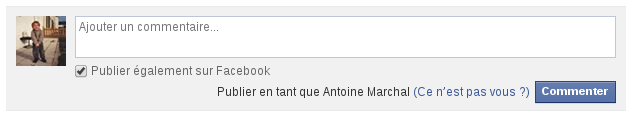
\includegraphics[scale=0.55]{figures/module_facebook_lalibre.png}
	\caption{\label{etag}Module de commentaires via Facebook sur \textit{lalibre.be}.}
\end{figure}

\begin{figure}[h]
	\centering
	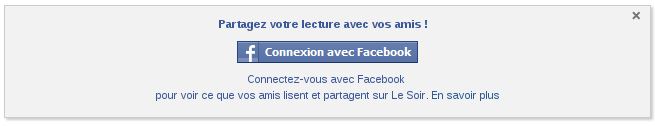
\includegraphics[scale=0.55]{figures/module_facebook_lesoir.png}
	\caption{\label{etag}Module incitant le visiteur à lier son compte Facebook au site \textit{lesoir.be}.}
\end{figure}

\subsubsection{Facebook}
Le code que les gestionnaires de sites Web doivent intégrer au sein de leur page afin d'accéder aux fonctionnalités offertes par Facebook \cite{javascript_facebook_sdk} est visible à la \autoref{js_facebook_sdk}. L'intégration de ce code permet aux sites Web d'utiliser entre autres les plugins suivants : le bouton "Like", le bouton de partage, le flux d'actualités d'une page Facebook et le module de commentaires.

Facebook propose également un SDK pour PHP et donne une liste de SDK, plugins et outils développés par d'autres. Les possibilités offertes par Facebook sont nombreuses, elles vont du module d'identification au module de paiements en passant par la publicité. Tout est bien détaillé sur un portail destiné aux développeurs \footnote{\url{https://developers.facebook.com/docs/}}.

\begin{figure}[h]
	\centering
	\lstinputlisting{examples/js_facebook_sdk}
	\caption{\label{js_facebook_sdk}Le SDK de \textit{Facebook} pour JavaScript}.
\end{figure}

\subsubsection{Google+}
De son côté, Google propose différents scripts à ajouter en fonction des fonctionnalités que le gestionnaire de site Web veut intégrer au sein de sa page (voir \autoref{js_google_plus}). Google propose même de charger de façon asynchrone son script afin d'obtenir des performances optimales (voir \autoref{js_google_plus_async}) \cite{javascript_google_plus}. Google+ propose le même genre de plugins \footnote{\url{https://developers.google.com/+/}} que Facebook tels que l'installation d'un module d'identification par compte Google, des boutons de partage, de recommandations, de suivi et autres.

\begin{figure}[h]
	\centering
	\lstinputlisting{examples/js_google_plus}
	\caption{\label{js_google_plus}L'API JavaScript de \textit{Google+}}.
\end{figure}

\begin{figure}[h]
	\centering
	\lstinputlisting{examples/js_google_plus_async}
	\caption{\label{js_google_plus_async}L'API JavaScript de \textit{Google+} pour un chargement asynchrone}.
\end{figure}

\subsubsection{LinkedIn}
LinkedIn propose également une API pour connecter les sites avec sa plateforme \cite{javascript_linkedin}. Dans la \autoref{js_linkedin}, on peut même voir que le nom de l'utilisateur (s'il est connecté sur la plateforme) est affiché sur le site. Cet aspect semblera convivial à la majorité des utilisateurs mais cela permet surtout de mieux les suivre lors de leur navigation sur les sites intégrant ce module social. Cette fonctionnalité est d'ailleurs également proposée par les autres plateformes de réseaux sociaux.

\begin{figure}[!h]
	\centering
	\lstinputlisting{examples/js_linkedin}
	\caption{\label{js_linkedin}L'API JavaScript de \textit{LinkedIn}}.
\end{figure}

\subsection{Outils destinés aux webmasters}
Certaines plateformes proposent aux gestionnaires de sites Web de suivre la navigation des visiteurs sur leur site. Elles regardent d'où viennent les visites (moteur de recherche, accès direct, lien d'un autre site,...), leur navigateur (la version, les extensions installées, la langue,...), sur quels pages les visiteurs se rendent, combien de temps ils restent sur chaque page, etc.

\subsubsection{Google Analytics (Universal Analytics)}
\label{google_analytics}
Une des principales plateformes de suivi des utilisateurs est Google Analytics. Cet outil est utilisé par de nombreux gestionnaires de sites afin de connaître les statistiques de fréquentation de leur site \cite{javascript_google_analytics}.

\begin{figure}[!h]
	\centering
	\lstinputlisting{examples/js_google_analytics}
	\caption{\label{js_google_analytics}L'API JavaScript de \textit{Google Analytics}}.
\end{figure}

Comme on peut le voir sur la \autoref{Google_Analytics_1}, les statistiques sont très détaillées. Dans la \autoref{Google_Analytics_2}, la ville des visiteurs était affichée mais il est également possible de voir d'autres données telles que leur FAI ou leur système d'exploitation. Des données spécifiques aux clients mobiles sont également disponibles. Toutes les données sont affichées dans des graphiques clairs et dynamiques et il est même possible d'exporter l'ensemble de ces données dans différents formats (CSV, TSV, Excel, PDF,...) afin de les traiter de manière automatique.
\newline

\begin{figure}[!h]
	\centering
	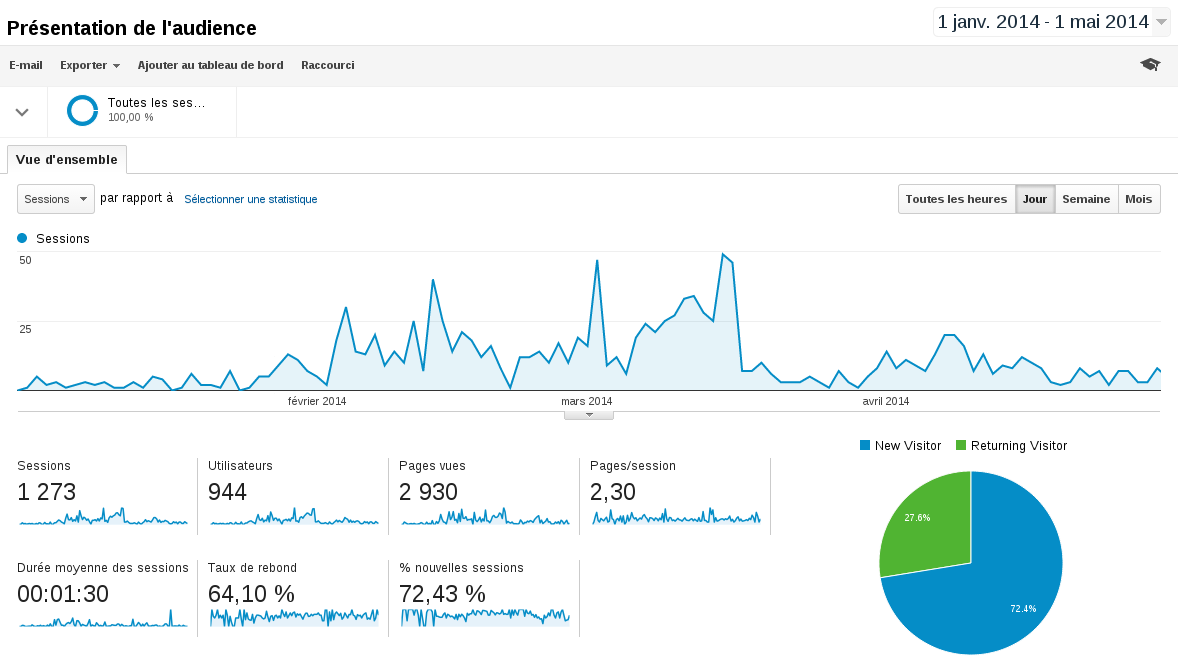
\includegraphics[scale=0.35]{examples/Google_Analytics_1.png}
	\caption{\label{Google_Analytics_1}Copie d'écran de \textit{Google Analytics} qui détaille les visites}
\end{figure}

\begin{figure}[!h]
	\centering
	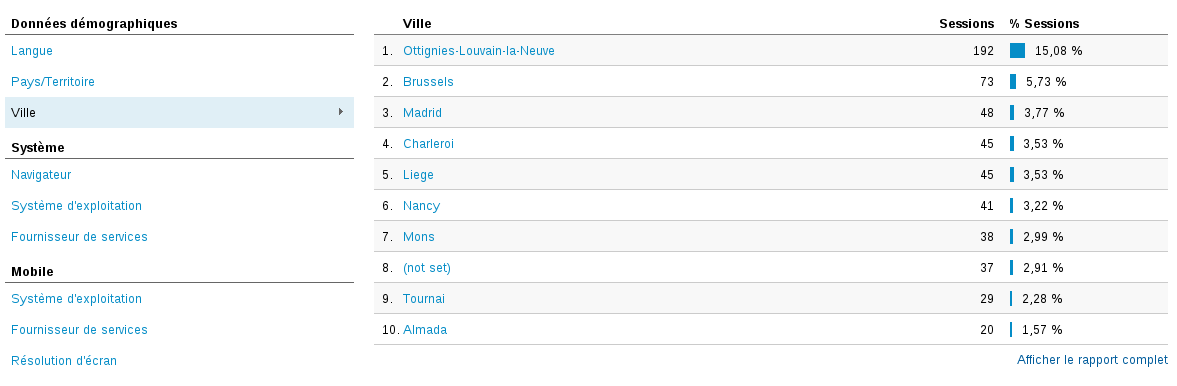
\includegraphics[scale=0.35]{examples/Google_Analytics_2.png}
	\caption{\label{Google_Analytics_2}Copie d'écran de \textit{Google Analytics} qui détaille l'origine des visiteurs}
\end{figure}

Google a développé une nouvelle version de son outil d'analyse des visiteurs : Universal Analytics. Ce nouvel outil repose sur le même socle que Google Analytics mais il apporte de nouvelles fonctionnalités.

Pour ce nouvel outil, Google propose 3 types de code de tracking en fonction des plateformes visées : la librairie JavaScript \textit{analytics.js} pour les sites Web, les SDK Google Analytics pour les applications mobiles et le \textit{protocole de mesure ("Measurement Protocol")} pour les autres appareils tels que consoles de jeux.% et les kiosques d'information.
\newline

Alors que Google Analytics identifiait un utilisateur différent en fonction de chaque appareil connecté, Universal Analytics reconnaît un même utilisateur qui utilise plusieurs moyens de se connecter à Internet. Afin d'y parvenir, ils utilisent un identifiant d'utilisateur unique afin d'associer les données reçues d'appareils et de sessions différentes.

Afin d'utiliser cette fonctionnalité, les gestionnaires de sites Web doivent être en mesure de générer un identifiant unique pour chaque utilisateur et l'associer aux données envoyées à Google. Généralement, cet identifiant unique est généré grâce à l'authentification des visiteurs sur un site. Ainsi, lorsqu'un utilisateur se sert de sa tablette et de son ordinateur pour se rendre sur un site et s'il s'y connecte, Google sera en mesure d'identifier ces visites comme provenant d'un seul et même utilisateur et non plus de deux utilisateurs différents.
\newline

En fonction de la version de Google Analytics utilisée, différents cookies sont créés et utilisés afin de suivre les visites des utilisateurs \cite{Google_Analytics_cookies}.
\newline

La nouvelle librairie JavaScript de Google, \textit{analytics.js} crée un cookie d'origine contenant un identifiant anonyme afin de distinguer les utilisateurs. Par défaut, la librairie crée un cookie sur le domaine de plus haut niveau et règle le chemin du cookie sur le niveau racine.

Le cookie créé est :
\begin{itemize}
  \item[$\bullet$] \textbf{\_ga} : cookie avec une date d'expiration de 2 ans destiné à distinguer les utilisateurs.
  \newline
\end{itemize}

L'ancienne libraire JavaScript de Google, \textit{ga.js}, crée 5 cookies d'origine qui permettent de :
\begin{itemize}
  \item déterminer quel domaine est mesuré
  \item distinguer les utilisateurs uniques
  \item se souvenir du nombre et des heures des visites précédentes
  \item se souvenir de l'information sur la source de trafic
  \item déterminer le début et la fin de session
  \item se souvenir des valeurs des variables personnalisées au niveau de l'utilisateur
\end{itemize}

Par défaut, la librairie crée un cookie sur le domaine spécifié dans la propriété du navigateur \textit{document.host} et règle le chemin du cookie sur le niveau racine.

Les cookies créés sont:
\begin{itemize}
  \item[$\bullet$] \textbf{\_\_utma} : cookie avec une date d'expiration de 2 ans destiné à distinguer les utilisateurs et les sessions.
  \item[$\bullet$] \textbf{\_\_utmb} : cookie avec une date d'expiration de 30 minutes destiné à distinguer les nouvelles sessions et visites.
  \item[$\bullet$] \textbf{\_\_utmc} : cookie avec une date d'expiration de fin de session qui n'est plus utilisé dans \textit{ga.js} mais qui permet l'interopérabilité avec \textit{urchin.js} (une librairie encore plus ancienne de Google Analytics, antérieure à \textit{ga.js}).
  \item[$\bullet$] \textbf{\_\_utmz} : cookie avec une date d'expiration de 6 mois destiné à enregistrer les sources de trafic ou de campagne qui explique comment un utilisateur atteint le site.
  \item[$\bullet$] \textbf{\_\_utmv} : cookie avec une date d'expiration de 2 ans utilisé pour sauvegarder les données des variables personnalisées au niveau de l'utilisateur.
  \newline
\end{itemize}

Avec le nombre élevé de sites utilisant les services de Google, ce dernier a les moyens de dresser une carte d'Internet. Il est même en mesure de connaître la plupart des sites visités de l'utilisateur (à la condition qu'ils intègrent un tracker de Google). Cela va sans dire que Google détient une très grande quantité d'informations sur les utilisateurs du Web actuel quand on y ajoute les messages privés (Gmail), la localisation (Android) et les nombreux autres services du groupe.

%%%%%%%%%%%%%%%%%%%%%%%%%%%%%%
\section{Flash}
\label{flash}
Adobe Flash Player \cite{flash_website} est un logiciel qui permet de lire du contenu multimédia. Il est notamment utilisé pour la conception de jeux sur Internet ou pour le streaming audio/vidéo (il était auparavant utilisé par YouTube qui a désormais décidé de se tourner vers la technologie HTML 5 \cite{youtube_html5}).
\newline

Flash peut être utilisé dans le tracking des utilisateurs car il utilise son propre système de cookies : les LSO (Local Shared Objects) \cite{conf/aaaiss/SoltaniCMTH10}. Ces derniers sont même considérés plus invasifs que les cookies HTTP car ils possèdent certaines caractéristiques \cite{flash_lso} :
\begin{itemize}
  \item ils permettent de stocker plus d'informations (100KB au lieu de 4KB pour les cookies HTTP)
  \item ils n'ont pas de date d'expiration par défaut
  \item ils sont stockés dans un emplacement différent, ce qui implique que la plupart des utilisateurs ne savent pas les effacer facilement et qu'ils sont accessibles via différents navigateurs
  \item ils ne sont pas contrôlés par le navigateur et celui-ci ne peut donc pas les effacer
  \item ils permettent de stocker des types de données simples (String, Array et Date)
  %\newline
\end{itemize}

Ces caractéristiques font que les cookies Flash (ce sont des fichiers avec l'extension \textit{.sol}) sont plus persistants et méconnus des utilisateurs. Pour supprimer les cookies Flash sans connaître leur emplacement, il faut se rendre sur une page dédiée \footnote{\url{http://www.macromedia.com/support/documentation/en/flashplayer/help/settings_manager07.html}} du site d'Adobe \footnote{Adobe est le développeur de Flash Player.}.
\newline

Le répertoire utilisé pour les stocker sur Linux est :\\
\mbox{\textit{/home/<user>/.macromedia/Flash\_Player}}. Celui-ci abrite deux répertoires :
\begin{enumerate}
  \item macromedia.com : il contient les paramètres de chaque site utilisant Flash.
  \item \#SharedObjects : il contient les LSO (les cookies Flash).
  %\newline
\end{enumerate}

Avec le contenu du répertoire \textit{macromedia.com}, on peut constater un autre risque de fuites concernant la vie privée : en analysant les traces laissées dans ce répertoire, il est possible de reconstituer une partie de l'historique de navigation de l'utilisateur. En effet, pour chaque domaine, un dossier est créé portant son nom et contenant un fichier de préférences \textit{settings.sol}. Simplement en regardant le nom des dossiers, il est possible de découvrir certains sites visités (voir \autoref{ls_macromedia.com}).

Notez que le navigateur Google Chrome n'utilise pas ce répertoire car Flash est intégré au navigateur \cite{flash_chrome}. Il est donc possible de supprimer les cookies Flash dans les paramètres du navigateur ou en se rendant sur la page dédiée du site Adobe.
\newline

\begin{figure}[h]
	\centering
	\lstinputlisting[style=dig]{examples/ls_macromedia.com}
	\caption{\label{ls_macromedia.com}Affichage des dossiers dans \textit{macromedia.com}}.
\end{figure}

Dans une expérience réalisée en 2009 \cite{conf/aaaiss/SoltaniCMTH10}, il a été montré que dans le TOP 100 des sites (classement Quantcast - juillet 2009), 54 sites ont utilisé des cookies Flash. Ces 54 sites ont généré 157 fichiers LSO pour arriver à un total de 281 cookies individuels. 98\% de ces sites ont également créé des cookies HTTP (seuls \textit{wikipedia.org} et \textit{wikimedia.org} ne l'ont pas fait) pour un total de 3602 cookies HTTP.

Ensuite, les chercheurs ont analysé les noms de variables les plus fréquemment utilisés dans ces cookies. Il en est ressorti que "volume" était en première position, ce qui fait penser à une préférence de volume pour le streaming (ce qui est logique car Flash reste avant tout un lecteur multimédia). Juste derrière et dans la majorité des cas, les noms de variables reflétaient l'idée d'identifiant (\textit{userid}, \textit{user}, \textit{id},...). Il est donc clair que les cookies Flash sont utilisés pour tracer les utilisateurs.

Le contenu des cookies Flash a été comparé avec le contenu des cookies HTTP. Sur les 100 sites, 31 montraient au moins un lien entre les cookies Flash et HTTP. Sur la totalité des 31 sites, 41 correspondances ont été trouvées.

Les chercheurs ont également montré que les cookies Flash étaient utilisés pour faire réapparaître les cookies HTTP lorsqu'ils étaient supprimés. Ainsi, certains sites recréaient les cookies HTTP grâce aux cookies Flash. Donc même si l'utilisateur effaçait les cookies HTTP via les préférences de son navigateur, les cookies de certains sites avec leur valeur étaient de nouveau envoyés lors des visites sur ces sites. Il faut également noter que certains cookies HTTP étaient recréés par des cookies Flash tiers.
\newline

En 2011, l'expérience a été menée à nouveau \cite{flash_cookies_privacy_2}. Cette fois, les chercheurs se sont penchés également sur le stockage local HTML5 (voir la \autoref{cache_html5}). Les résultats sont les suivants : 5675 cookies HTTP ont été détectés (au lieu de 3602 en 2009). 20 sites ont placé 100 cookies ou plus et 7 sites en ont placé plus de 150. La plupart des noms de variables de ces cookies font penser à un identifiant unique de tracking. La plupart des cookies (4915) sont placés par un domaine tiers.

Concernant les cookies Flash, ils sont en baisse car 100 ont été détectés (au lieu de 281 en 2009) sur 37 sites (au lieu de 54 en 2009).
Deux sites (hulu.com et foxnews.com) utilisaient des valeurs communes dans leurs cookies Flash et HTTP, la valeur était également commune dans le stockage local HTML5.
\newline

Il faut noter qu'Adobe a condamné l'utilisation des LSO à des fins de tracking. L'entreprise incite les développeurs à utiliser la technologie Flash de manière responsable et de ne pas utiliser de technique qui permette d'utiliser le stockage local afin de récréer des cookies effacés par l'utilisateur sans leur consentement \footnote{La déclaration complète d'Adobe est disponible à l'URL suivante : \url{http://www.ftc.gov/policy/public-comments/comment-544506-00085}}. Ils détaillent également quelques nouveautés qui seront ajoutées aux prochaines versions de Flash (notamment le support de la navigation privée).
\newline

Avant la version 10.1 de Flash Player \cite{flash_private}, celui-ci ne prenait pas en compte les effets des sessions de navigation privée des navigateurs. Cela signifie que lorsqu'un utilisateur activait une session de navigation privée avec son navigateur, les cookies, fichiers en cache et l'historique de sa session étaient supprimés par le navigateur mais ce n'était pas le cas pour les cookies Flash. Depuis la version 10.1 de Flash Player, celui-ci garde les fichiers LSO de la navigation privée en mémoire sans les enregistrer sur le disque et n'accède pas non plus aux LSO existants. A la fin de la session de navigation privée, Flash Player efface les données en conformité avec les préférences du navigateur.

%%%%%%%%%%%%%%%%%%%%%%%%%%%%%%
\section{Empreintes des navigateurs}
\label{fingerprinters}
Jusqu'à présent, nous avons vu des techniques de tracking dites avec état (stateful tracking). A l'opposé, il existe des techniques dites sans état (stateless tracking) utilisant des \textit{fingerprinters\footnote{En français, on pourrait traduire ce mot par "calculateur d'empreinte".}} \cite{Mayer:2012:TWT:2310656.2310703}. Ces derniers récupèrent une série d'informations qu'ils agrègent afin d'associer un identifiant (presqu') unique à l'utilisateur. Le principal avantage de cette méthode est que les informations ne dépendent que très peu de l'utilisateur.
En effet, avec des techniques utilisant des cookies, le tracking peut être rendu complexe par la suppression des cookies par l'utilisateur. A l'inverse, avec les fingerprinters, les informations récupérées sont relativement stables grâce à leur nature (numéro de version du navigateur, système d'exploitation, la résolution d'écran, etc).
\newline

Le \textit{fingerprinter} regroupe les informations qui lui sont nécessaires via différentes sources \cite{Nikiforakis:2013:CME:2497621.2498133}. La première source est constituée des plugins populaires tels que Flash. Par exemple, lorsqu'on demande au navigateur la plateforme d'exécution sur une version 64 bits de Linux, il répond "Linux x86\_64" alors que si on demande la même information à Flash, il répond en indiquant la version complète du noyau Linux. Il est également possible de déterminer si l'utilisateur utilise un second écran. En effet, avec l'implémentation Linux du plugin Flash, lorsque la résolution est demandée, Flash renvoie comme résolution d'écran la somme des écrans individuels alors que le navigateur renvoie la résolution de l'écran sur lequel la fenêtre est affichée.

Les outils de fingerprinting s'adaptent également aux navigateurs des utilisateurs. Il a été montré qu'ils utilisent des propriétés spécifiques à certains navigateurs afin de récupérer certaines données. C'est notamment le cas avec Internet Explorer et les propriétés \textit{navigator.securityPolicy} et \textit{navigator.systemLanguage} \cite{Nikiforakis:2013:CME:2497621.2498133}.

Une autre source importante d'informations vient des polices de caractères utilisées. Cette information n'est pas directement disponible via les navigateurs et les \textit{fingerprinters} n'hésitent pas à utiliser des plugins comme Flash pour récupérer cette liste. De plus, certains \textit{fingerprinters} incluent un "plan B" lorsque Flash n'est pas disponible. Ils mesurent la taille d'un phrase prédéfinie avec la police utilisée par défaut si la police demandée n'est pas disponible puis ils appliquent une police différente et mesurent la taille de la même phrase. Si la taille est identique, cela veut dire que la police n'est pas disponible chez l'utilisateur. Ils sont ainsi en mesure de déterminer une liste de polices installées chez l'utilisateur (avec l'inconvénient que les polices les plus rares ne sont pas détectées). Il faut noter que la présence de certaines polices rares permettent d'identifier un utilisateur avec une précision beaucoup plus importante \cite{Boda:2011:UTW:2341491.2341497}.

Flash est également utilisé pour détecter les proxys HTTP. C'est d'ailleurs la raison pour laquelle il est désactivé dans des applications sensibles à l'anonymat.

Une dernière source utilisée dans Internet Explorer provient des DLL chargées dans le navigateur. Certaines accèdent à des valeurs du registre Windows afin de transmettre des informations telles que les identifiants des disques durs, des paramètres TCP/IP, le nom de l'ordinateur, identifiant de produit d'Internet Explorer, la date d'installation de Windows, l'ID produit Windows Digital et les pilotes installés \cite{Nikiforakis:2013:CME:2497621.2498133}.
\newline

Au sein du tracking sans état, on peut distinguer deux types d'utilisation du \textit{fingerprinting} : le \textit{fingerprinting actif} qui acquiert les informations de manière active grâce à l'utilisation de scripts ou de plugins et le \textit{fingerprinting passif} qui acquiert les informations de manière passive grâce au trafic réseau (les requêtes et réponses HTTP).
Le \textit{fingerprinting passif} est particulièrement problématique car il n'est pas détectable par le client. Un fingerprinter n'utilisant que du fingerprinting passif sera moins performant mais sera néanmoins en mesure de tracer certains types d'utilisateurs qui utilisent un navigateur qui est rarement modifié et peu mis à jour
\newline

Un aspect intéressant à analyser est la stabilité des empreintes des navigateurs. En effet, l'empreinte d'un navigateur peut être modifiée par différentes actions : mettre à jour le navigateur, mettre à jour un plugin, désactiver les cookies, installer une nouvelle police de caractères ou application qui contient des polices ou connecter un second moniteur (ce qui change la résolution d'écran). Il semblerait que les empreintes calculées ne soient pas particulièrement stables mais le fait que le navigateur dévoile tant d'informations rend cette technique de tracking très intéressante. \cite{Eckersley:2010:UYW:1881151.1881152}

%%%%%%%%%%%%%%%%%%%%%%%%%%%%%%
\section{Conclusion}
Les moyens existants et mis en place dans le but de tracker les utilisateurs sont nombreux et divers. Certains restent relativement basiques alors que d'autres utilisent des techniques plus complexes. Certains sont conçus principalement dans le but d'effectuer un tracking sur un site particulier (les outils d'analyses de visites) alors que d'autres sont destinés à tracer les visiteurs sur de multiples sites (les régies publicitaires) afin de créer un profil des visiteurs.

Il semble que les possibilités et moyens de tracker les utilisateurs naviguant sur Internet évoluent rapidement. De nouvelles techniques apparaissent alors que d'autres sont peu à peu oubliées.
